\documentclass[24pt]{beamer}
\usepackage[utf8]{inputenc}
\usepackage[utf8]{vietnam}
\usepackage{amsmath}
\usepackage{amsfonts}
\usepackage{amssymb}
\usepackage{graphicx}
\usepackage{multimedia}
\usepackage{tikz}
\usetikzlibrary{positioning}
\usetikzlibrary{arrows}
\usetikzlibrary{decorations.markings}
\usepackage{xcolor}
\usepackage{utopia} %font utopia imported
\usepackage{siunitx}
\usepackage[american,cuteinductors,smartlabels]{circuitikz}
\usepackage{ragged2e}
\usepackage{etoolbox}

\mode<beamer>{\usetheme{CambridgeUS}}

\usecolortheme{default}

\usepackage{hyperref}
\hypersetup{pdfpagemode=FullScreen} %mode FullScreen with beamer

\apptocmd{\frame}{}{\justifying}{} % Allow optional arguments after frame.

\usepackage{comment}

\makeatletter
\let\insertuniversity\relax
\newcommand\universitytitle{TRƯỜNG ĐH}

\let\insertclass\relax
\newcommand\classtitle{Lớp}

\let\insertcourse\relax
\newcommand\coursetitle{Môn học}

\mode<all>
{
  \newcommand\university[1]{\def\insertuniversity{#1}}
  
  \newcommand\class[1]{\def\insertclass{#1}}
  
  \newcommand\course[1]{\def\insertcourse{#1}}
  \titlegraphic{}
}

\defbeamertemplate*{title page}{supdefault}[1][]
{
  \begingroup
    \centering
    \ifx\insertuniversity\relax\relax\else
    \begin{beamercolorbox}[sep=2pt,center,#1]{author}
      \hspace{-.15cm}\scriptsize\universitytitle~\insertuniversity
    \end{beamercolorbox}\fi
    
    \begin{beamercolorbox}[sep=8pt,center,#1]{title}
      \usebeamerfont{title}\normalsize\inserttitle\par%
      \ifx\insertsubtitle\@empty\relax%
      \else%
        \vskip0.25em%
        {\usebeamerfont{subtitle}\usebeamercolor[fg]{subtitle}\insertsubtitle\par}%
      \fi%     
    \end{beamercolorbox}%
    \vskip.5em\par

    \vspace{-.4cm}
    \ifx\insertcourse\relax\relax\else
    \begin{beamercolorbox}[sep=6pt,center,#1]{author}
      \usebeamerfont{author}\footnotesize\coursetitle:~\insertcourse
    \end{beamercolorbox}\fi

    \vspace{-.3cm}
    \ifx\insertclass\relax\relax\else
    \begin{beamercolorbox}[sep=6pt,center,#1]{author}
      \usebeamerfont{author}\footnotesize\classtitle:~\insertclass
    \end{beamercolorbox}\fi

    \vspace{-.3cm}
    \begin{beamercolorbox}[sep=6pt,center,#1]{author}
      \usebeamerfont{author}\hspace{-.23cm}\footnotesize\insertauthor
    \end{beamercolorbox}
    %\begin{beamercolorbox}[sep=8pt,center,#1]{institute}
      %\usebeamerfont{institute}\insertinstitute
    %\end{beamercolorbox}
    \vspace{-.4cm}
    \begin{beamercolorbox}[sep=8pt,center,#1]{date}
      \usebeamerfont{date}\footnotesize\insertdate
    \end{beamercolorbox}\vskip0.5em
    {\usebeamercolor[fg]{titlegraphic}\inserttitlegraphic\par}
  \endgroup
  \vfill
}
\setbeamertemplate{title page}[supdefault][colsep=-4bp,rounded=true,shadow=\beamer@themerounded@shadow]\makeatother

%Title page
\title[Động cơ điện một chiều]{\emph{Chủ đề báo cáo}\\ Hãm động cơ DC và Thay đổi tốc độ vòng hở từ nguồn DC}
\author[Cơ sở Truyền động điện]{GVHD: Hồ Minh Nhị \and Nhóm SVTH: Nhóm 1}
\course{Cơ sở Truyền động điện}
\class{Công nghệ, kỹ thuật điện, điện tử}
\university{KỸ THUẬT -- CÔNG NGHỆ CẦN THƠ}
\date[Nhóm 1]{\today}

%\logo{
\includegraphics[height=1.3cm]{logo_ctut.pdf}}

\AtBeginSection[]
{
  \begin{frame}
    \frametitle{Nội dung báo cáo}
    \justifying
    \tableofcontents[currentsection]
  \end{frame}
}
\definecolor{doden}{RGB}{204, 0, 0}
\newcommand{\noibat}[1]{\textcolor{red}{#1}}
\newcommand{\noibatn}[1]{\textcolor{blue}{#1}}
\newcommand{\drawe}{\draw[line width=1.2pt]}
\newcommand{\pfm}[1]{\left({#1}\right)}
\newcommand{\viet}[2]{#1_{\text{\textit{#2}}}}
\begin{document}
%http://tex.stackexchange.com/questions/82794/removing-page-number-from-title-frame-without-changing-the-theme
\bgroup
\makeatletter
\setbeamertemplate{footline}
{
  \leavevmode%
  \hbox{%
  \begin{beamercolorbox}[wd=.333333\paperwidth,ht=2.25ex,dp=1ex,center]{author in head/foot}%
    \usebeamerfont{author in head/foot}\insertshortauthor\expandafter\beamer@ifempty\expandafter{\beamer@shortinstitute}{}{~~(\insertshortinstitute)}
  \end{beamercolorbox}%
  \begin{beamercolorbox}[wd=.333333\paperwidth,ht=2.25ex,dp=1ex,center]{title in head/foot}%
    \usebeamerfont{title in head/foot}\insertshorttitle
  \end{beamercolorbox}%
  \begin{beamercolorbox}[wd=.333333\paperwidth,ht=2.25ex,dp=1ex,right]{date in head/foot}%
    \usebeamerfont{date in head/foot}\insertshortdate{}\hspace*{2em}
%    \insertframenumber{} / \inserttotalframenumber\hspace*{2ex} 
    \hspace*{6ex}
  \end{beamercolorbox}}%
  \vskip0pt%
}

\begin{frame}
\titlepage
\end{frame}
\egroup

\setcounter{framenumber}{0}

%--------------------------------------------------------------------------------
%--------------------------------------------------------------------------------
% Danh sách thành viên
\begin{frame}{Danh sách thành viên}
%	\vspace{-1cm}
	\begin{footnotesize}
	\begin{columns}
		\column{0.6\textwidth}
		\begin{enumerate}
			\item Nguyễn Văn Bảy
			\item Nguyễn Văn Đình
			\item Nguyễn Hoàng Hận
			\item Thi Minh Nhựt
			\item Phạm Thanh Quý
			\item Hồ Minh Thành
			\end{enumerate}

		\column{.6\textwidth}
		\begin{enumerate}	% Danh sach tiep theo
			\setcounter{enumi}{6}
			\item Nguyễn Văn Tiến
			\item Liên Thái Trường
			\item Trần Thanh Tú
			\item Bùi Trọng Tuấn
			\item Lư Anh Tuấn
			\item Nguyễn Bá Vọng
		\end{enumerate}
	\end{columns}
	\end{footnotesize}
\end{frame}

%--------------------------------------------------------------------------------
%--------------------------------------------------------------------------------
% Nội dung báo cáo
\begin	{frame}	%Trang muc luc
	\frametitle{Nội dung báo cáo}
	\tableofcontents
\end{frame}

%--------------------------------------------------------------------------------
%--------------------------------------------------------------------------------
% Hãm động cơ DC
\section{Hãm động cơ DC}
\subsection*{Các chế độ hãm động cơ DC}
\begin{frame}{Chế độ hãm động cơ DC}
\justifying
ĐC DC kích từ độc lập hoặc kích từ nối tiếp, có 3 chế độ hãm ĐC: \vspace{-1cm}
\begin{itemize}
\item Hãm tái sinh.
\item Hãm động năng.
\item Hãm ngược.
\end{itemize}
\end{frame}

\section*{Hãm động cơ DC kích từ độc lập}
\subsection*{Hãm tái sinh}
\begin{frame}{Điều kiện hãm tái sinh}
\justifying
\alert{Điều kiện:} $E > U$ $\rightarrow$ cơ năng chuyển thành điện năng trả về nguồn. \alert{ĐC hoạt động ở chế độ máy phát} (vùng $II$).

\alert{Lưu ý:} Nguồn $U$ phải có khả năng nhận năng lượng.
\end{frame}

\begin{frame}{Trường hợp hãm tái sinh}
\justifying
\alert{Nguồn $U$ không đổi:} điều kiện xảy ra $\omega_{\text{\textit{tải}}} > \omega_{\text{\textit{không tải}}}$ $\rightarrow$ không dừng được động cơ.

\alert{Nguồn $U$ thay đổi:} dùng để điều khiển giảm tốc hoặc dừng ĐC.
\end{frame}

\begin{frame}{Đặc tính cơ}
\vspace{-1.4cm}
	\begin{center}
		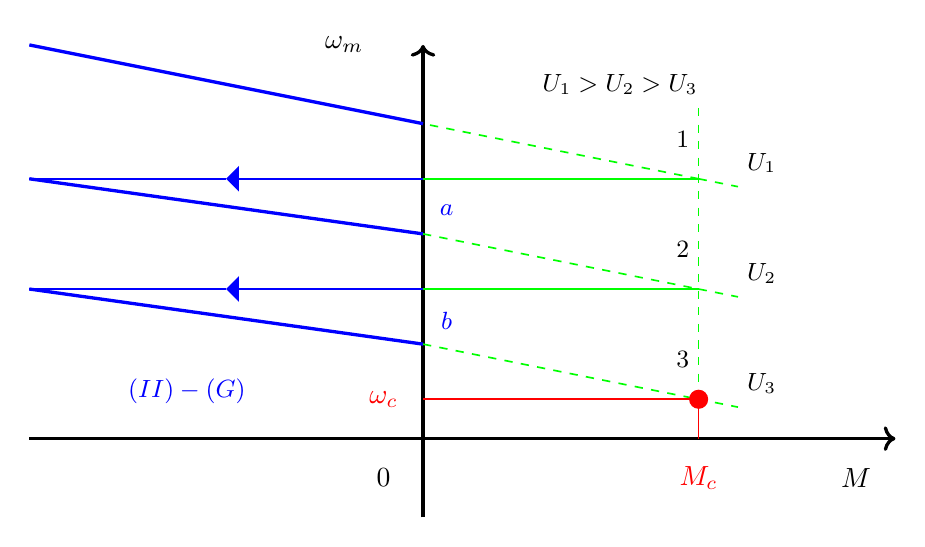
\begin{tikzpicture}
			\drawe[->] (-5,0) -- (6,0);
			\drawe[->] (0,-1) -- (0,5);

			\draw[dashed,green, line width=.6pt] (3.5,3.3) -- (0,4);
			\draw[dashed,green, line width=.6pt] (3.5,3.3) -- (4,3.2);
			\drawe[blue] (0,4) -- (-5,5);
			
			\draw[green, line width=.6pt] (3.5,3.3) -- (0,3.3);
			\drawe[blue,-triangle 90,fill=blue, line width=.6pt] (0,3.3) -- (-2.5,3.3);
			\drawe[blue, line width=.6pt] (-2.5,3.3) -- (-5,3.3);
			
			\drawe[blue] (-5,3.3) -- (0,2.6);
			\draw[dashed,green, line width=.6pt] (0,2.6) -- (3.5,1.9);
			\draw[dashed,green, line width=.6pt] (3.5,1.9) -- (4,1.8);
			
			\draw[green, line width=.6pt] (3.5,1.9) -- (0,1.9);
			\drawe[blue,-triangle 90,fill=blue, line width=.6pt] (0,1.9) -- (-2.5,1.9);
			\drawe[blue, line width=.6pt] (-2.5,1.9) -- (-5,1.9);
			
			\drawe[blue] (-5,1.9) -- (0,1.2);
			\draw[dashed,green, line width=.6pt] (0,1.2) -- (3.5,.5);
			\draw[dashed,green, line width=.6pt] (3.5,.5) -- (4,.4);
			
			\draw[dashed, green, line width=.6pt] (3.5,4.2) -- (3.5, .5);
			\draw[red, line width=.6pt] (3.5,.5) -- (3.5, 0);
			\draw[red, line width=.6pt] (3.5,.5) -- (0, 0.5);
			\drawe[red, fill=red] (3.5,.5) circle (.1);
			
			
			\draw (-1,5) node {$\omega_m$};
			\draw (-.5,-.5) node {$0$};
			\draw (5.5,-.5) node{$M$};
			\draw (3.5,-.5) node{$\textcolor{red}{M_{c}}$};
			\draw (-.5,.5) node{$\textcolor{red}{\omega_{c}}$};
			
			\draw (3.3,3.8) node {\small{$1$}};
			\draw (4.3,3.5) node {\small{$U_1$}};
			
			\draw (3.3,2.4) node {\small{$2$}};
			\draw (4.3,2.1) node {\small{$U_2$}};
			
			\draw (3.3,1) node {\small{$3$}};
			\draw (4.3,.7) node {\small{$U_3$}};
			
			\draw (.3,2.9) node {\small{\textcolor{blue}{$a$}}};
			\draw (.3,1.5) node {\small{\textcolor{blue}{$b$}}};
			
			\draw (-3,.6) node {\small{\textcolor{blue}{$(II) - (G)$}}};
			
			\draw (2.5,4.5) node {\small{$U_1 > U_2 > U_3$}};
		\end{tikzpicture}
	\end{center}
\end{frame}

\subsection*{Hãm động năng}
\begin{frame}{Hãm động năng}
	\vspace{-.4cm}
	\begin{center}
		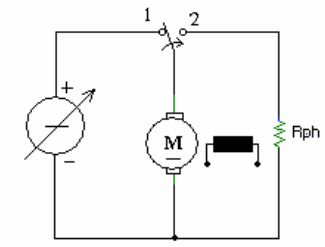
\includegraphics[scale=.65]{images-chude5/ham-dong-nang-doc-lap.png} 
	\end{center}
\end{frame}

\begin{frame}{Giải thích}
\justifying
Khi xảy ra quá trình hãm \alert{phần ứng} của ĐC nối với \alert{điện trở phụ} $\rightarrow$ năng lượng tiêu hao trên \alert{$R_{ph}$} và \alert{$\viet{R}{ư}$}.
\end{frame}

\subsection*{Hãm ngược}
\begin{frame}{Hãm ngược khi nguồn DC đổi dấu}
\vspace{-.4cm}
	\begin{center}
		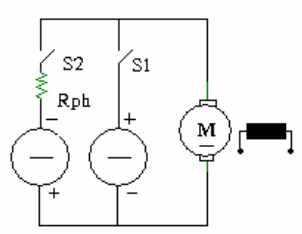
\includegraphics[scale=.6]{images-chude5/ham-nguoc-dc-doi-dau.png} 
	\end{center}
\end{frame}

\begin{frame}{Hãm ngược khi nguồn DC đổi dấu}
\justifying
Khi \alert{đảo vị trí dây nguồn} nối vào \alert{phần ứng} thì \alert{$E, U$ cùng dấu} tạo \alert{dòng điện hãm lớn} $\rightarrow$ \alert{mắc thêm điện trở phụ}.
\end{frame}

\begin{frame}{Hãm ngược khi nguồn DC không đổi dấu}
\justifying
Xảy ra khi thực hiện \alert{thải tải trọng}, làm \textcolor{blue}{vận tốc động cơ} \alert{ngược chiều} với \textcolor{blue}{vận tốc không tải}.
\end{frame}
%--------------------------------------------------------------------------------
%--------------------------------------------------------------------------------
% Hệ truyền động Chopper
\section[Hệ truyền động Chopper]{Thay đổi tốc độ vòng hở từ nguồn DC}
\subsection*{Các bộ biến đổi}
\begin{frame}{Hệ truyền động Chopper}
	\begin{itemize}
		\justifying
		\item Bộ giảm áp và tăng áp.
		\item Bộ biến đổi điện trở.		
		\item Bộ biến đổi kép đảo dòng và đảo áp.
		\item Bộ biến đổi kép tổng quát.
		\item Mạch lọc nguồn.
	\end{itemize}
\end{frame}
\subsection*{Bộ giảm áp}
\begin{frame}{Bộ giảm áp}
	\vspace{-.4cm}
	\begin{center}
		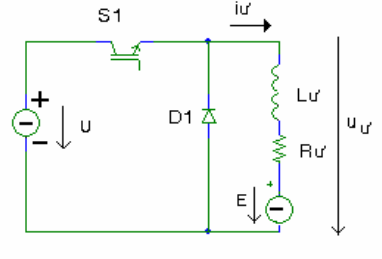
\includegraphics[scale=.7]{images-chude5/bo-giam-ap.png} 
	\end{center}
\end{frame}

\begin{frame}{Áp dụng}
\justifying
\alert{Chế độ hãm động cơ:} Sử dụng \alert{bộ giảm áp} kết hợp với \alert{hãm động năng} hoặc \alert{sự cản của tải} để dừng động cơ.

Điện áp tải: \alert{$U_t = U_d\dfrac{T_{on}}{T}$}
\end{frame}

\subsection*{Bộ tăng áp}
\begin{frame}{Bộ tăng áp}
	\vspace{-.4cm}
	\begin{center}
		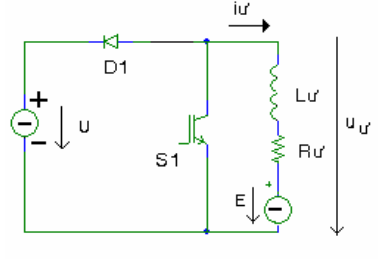
\includegraphics[scale=.7]{images-chude5/bo-tang-ap.png} 
	\end{center}
\end{frame}

\begin{frame}{Áp dụng}
\justifying
\alert{Bộ tăng áp} được áp dụng cho chế độ \alert{hãm tái sinh}.

Điện áp tải: \alert{$U_t = U_d\pfm{1 - \dfrac{T_{on}}{T}}$}
\end{frame}

\subsection*{Bộ biến đổi điện trở}
\begin{frame}{Bộ biến đổi điện trở}
	\vspace{-.5cm}
	\begin{center}
		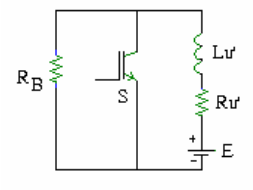
\includegraphics[scale=.9]{images-chude5/bo-bien-doi-dien-tro.png} 
	\end{center}
\end{frame}

\begin{frame}{Giải thích}
\justifying
	\alert{Đóng khóa S:} năng lượng tổn hao trên $\viet{R}{ư}$ và tích lũy trên $\viet{L}{ư}$.
	
	\alert{Ngắt khóa S:} năng lượng trên $\viet{L}{ư}$ và $E$ chuyển thành tổn hao trên $\viet{R}{ư}$ và $R_B$.
\end{frame}

\subsection*{Bộ biến đổi kép đảo dòng}
\begin{frame}{Bộ BĐ kép đảo dòng}
	\vspace{-.4cm}
	\begin{center}
		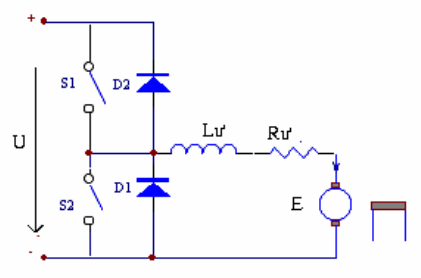
\includegraphics[scale=.65]{images-chude5/bo-bien-doi-dao-dong.png} 
	\end{center}
\end{frame}

\begin{frame}{Áp dụng}
\justifying
\alert{Áp dùng:} dùng điều khiển vận tốc động cơ kích từ độc lập.

\alert{Chế độ điều khiển:}

+ Chế độ ĐC: đóng $S_1$, ngắt $S_2$.

+ Chế độ hãm: đóng $S_2$, ngắt $S_1$.
\end{frame}

\subsection*{Bộ biến đổi kép tổng quát}
\begin{frame}{Bộ BĐ kép tổng quát}
	\vspace{-.4cm}
	\begin{center}
		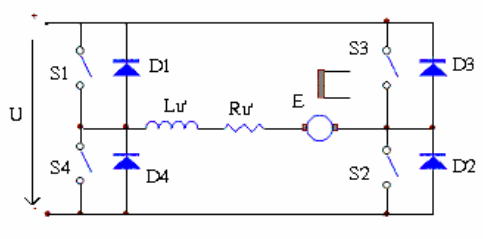
\includegraphics[scale=.65]{images-chude5/bo-bien-doi-tong-quat.png} 
	\end{center}
\end{frame}

\begin{frame}{Nguyên tắc điều khiển}
\justifying
Đóng $S_1S_2$ hoặc đóng $S_3S_4$ (\alert{kích đóng đối nghịch}).
\end{frame}

\subsection*{Mạch lọc}
\begin{frame}{Mạch lọc}
	\vspace{-.4cm}
	\begin{center}
		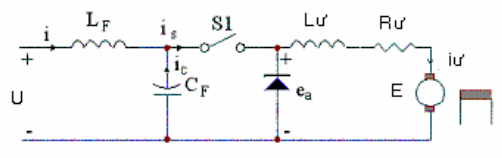
\includegraphics[scale=.65]{images-chude5/mach-loc.png} 
	\end{center}
\end{frame}

\begin{frame}{Giải thích}
\justifying
Do điện áp nguồn có dạng \alert{băm xung} chứa thành phần \alert{sóng hài} và \alert{tín hiệu nhiễu} nên cần sử dụng \alert{mạch lọc}.
\end{frame}
%--------------------------------------------------------------------------------
%--------------------------------------------------------------------------------
% Tài liệu tham khảo
\section*{Tài liệu tham khảo}
\begin{frame}{Tài liệu tham khảo}
\begin{small}
\justifying
[1]. Nguyễn Văn Nhờ, \textit{Cơ sở Truyền động điện}, NXB ĐH Quốc gia HCM.

[2]. Nguyễn Văn Nhờ, \textit{Điện tử công suất 1}, NXB ĐH Quốc gia HCM.
\end{small}
\end{frame}
%--------------------------------------------------------------------------------
%--------------------------------------------------------------------------------
% Lời cảm ơn
\section*{Lời cảm ơn}
\begin{frame}
\justifying
\large \alert{Cảm ơn Thầy và các bạn đã quan tâm theo dõi phần trình bày của nhóm!}
\end{frame}
\end{document}